\section{Correlation}\label{sec:corr}

One approach to understanding how different zero-cost proxies relate to the validation accuracy of the architecture is by calculating the correlation. Spearman Rank Correlation is a non-parametric statistical test that measures the strength and direction of the association between two ranked variables \autocite{hauke2011comparison}. The Spearman Rank does not assume a linear relationship between the two variables. However, it measures the strength of a monotonic relationship, which makes it suitable for cases where the relationship between the zero-cost proxy and the validation accuracy might not be linear. In addition, the metric is less sensitive to outliers since it relies on the rank of the variables rather than their raw values. This property makes the metric more robust when dealing with noisy or imprecise data, which can be expected in the context of zero-cost proxies. 

It is denoted by the symbol $\rho$ (rho) and ranges from -1 to 1, where -1 indicates a perfect negative relationship, 1 indicates a perfect positive relationship, and 0 shows no connection, as illustrated in \cref{fig:correlations_illustrated} \autocite{laerdstatistics}.  

\begin{figure}[h]
\centering
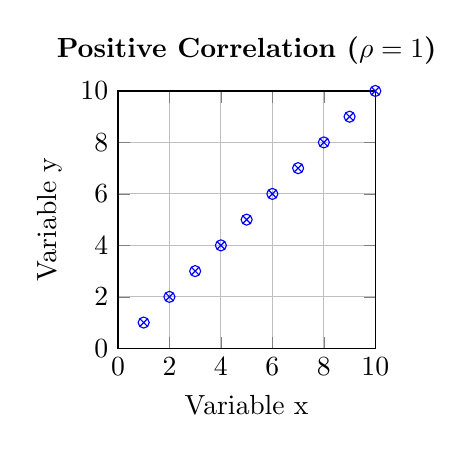
\begin{tikzpicture}
\begin{axis}[
    title={\textbf{Positive Correlation ($\rho = 1$)}},
    xlabel={Variable x},
    ylabel={Variable y},
    xmin=0, xmax=10,
    ymin=0, ymax=10,
    xtick={0,2,4,6,8,10},
    ytick={0,2,4,6,8,10},
    grid=major,
    legend pos=south east,
    width=0.4\textwidth,
    height=0.4\textwidth,
]
\addplot[
    only marks,
    mark=otimes,
    color=blue,
] coordinates {
(1,1)(2,2)(3,3)(4,4)(5,5)(6,6)(7,7)(8,8)(9,9)(10,10)
};
\end{axis}
\end{tikzpicture}
\hspace{1cm}
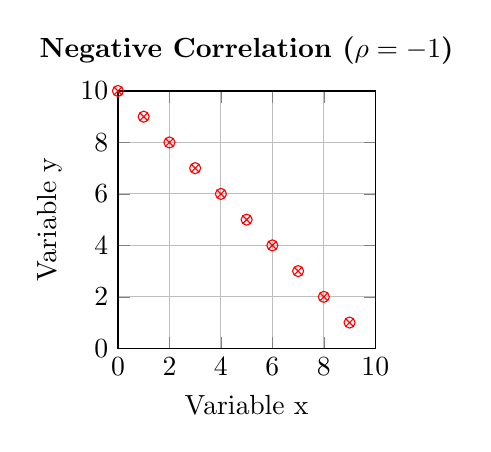
\begin{tikzpicture}
\begin{axis}[
    title={\textbf{Negative Correlation ($\rho = -1$)}},
    xlabel={Variable x},
    ylabel={Variable y},
    xmin=0, xmax=10,
    ymin=0, ymax=10,
    xtick={0,2,4,6,8,10},
    ytick={0,2,4,6,8,10},
    grid=major,
    legend pos=south east,
    width=0.4\textwidth,
    height=0.4\textwidth,
]
\addplot[
    only marks,
    mark=otimes,
    color=red,
] coordinates {
(9,1)(8,2)(7,3)(6,4)(5,5)(4,6)(3,7)(2,8)(1,9)(0,10)
};
\end{axis}
\end{tikzpicture}
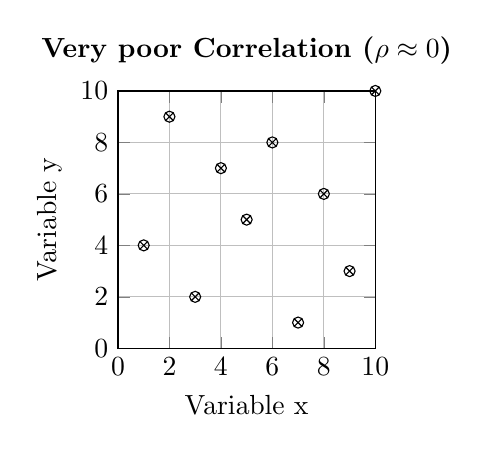
\begin{tikzpicture}
\begin{axis}[
    title={\textbf{Very poor Correlation ($\rho \approx 0$)}},
    xlabel={Variable x},
    ylabel={Variable y},
    xmin=0, xmax=10,
    ymin=0, ymax=10,
    xtick={0,2,4,6,8,10},
    ytick={0,2,4,6,8,10},
    grid=major,
    legend pos=south east,
    width=0.4\textwidth,
    height=0.4\textwidth,
]
\addplot[
    only marks,
    mark=otimes,
    color=black,
] coordinates {
(1,4)(2,9)(3,2)(4,7)(5,5)(6,8)(7,1)(8,6)(9,3)(10,10)
};
\end{axis}
\end{tikzpicture}

\caption{Scatter plots illustrating perfect positive, perfect negative correlations and very poor correlation}
\label{fig:correlations_illustrated}
\end{figure}

Spearman Rank Correlation works by calculating the difference in ranks of the two variables for each observation, then squaring these differences and summing them up. Mathematically, it is defined as: 

\begin{equation} 
\rho = 1 - \frac{6 \sum d_i^2}{n(n^2 - 1)}, 
 \end{equation}

where $d_i$ is the difference in ranks for each observation, and $n$ is the number of observations.

In the context of zero-cost proxies and validation accuracy, Spearman Rank Correlation can be used to determine whether there is a monotonic relationship between the two. A positive correlation would indicate that as the zero-cost proxy improves, so does the validation accuracy, while a negative correlation would imply an inverse relationship. A correlation near zero would suggest that the two variables have little or no association. 



